\documentclass[12pt,fleqn]{article}\usepackage{../../common}
\begin{document}
Dalga Denklemi (Wave Equation)

Denklem [1],

$$
\frac{\partial^2 y}{\partial x^2}  =
\frac{1}{c^2}\frac{\partial^2 y}{\partial t^2}
$$

Denkleme yakından bakarsak onun bir kısmı türevsel denklem (PDE) olduğunu
görürüz. İki tane bağımsız değişken temel alınıyor, $x,t$. Ayrıca denklem
2. derece, çünkü ikinci türevi içeriyor. Bu bilgiler denklemi çözmek için
önemli [2].

Çözümde bir başlangıç şartı gerekli çünkü diferansiyel denklemleri ``entegre
ederken'' daha doğrusu ileri doğru geçen zamanda hesaplarken bir başlangıç
noktası gerekiyor, bunun için bir teli kaldırıp (geçici bir süre üçgen haline
getirip) oradan bıraktığımızı düşünebiliriz, ki bu üçgen şekli alttaki gibi
modellenebilir,

$$
y(x,t=0)=\begin{cases}
1.25 x/L , &x\leq 0.8 L ,\\
(5-5x/L), &x> 0.8 L,
\end{cases} 
$$

İkinci bir başlangıç şartı daha lazım, 2. derece başlangıç şartı bu. Teli, ipi
gerip üçgen yaptım ama sonra durup tekrar bıraktım, bu da bir başlangıç şartı,
durağan durumdan başlama şartı.

$$
\frac{\partial y} {\partial t}(x,t=0) =0
$$

Çözüme bu şartlarla başlayabilirdik ama baştaki problem tanımını hatırlarsak ek
bazı şartlar daha koymuştuk, bu şartlar, kısıtlamalar her an için geçerli,
ipler iki ucundan (hareket etmeyen) duvarlara bağlı.

$$
y(0,t) \equiv 0, \quad y(L,t) \equiv 0
$$

[analitik çözüm atlandı]

Yaklaşıksal hesap için $x,t$ eksenleri düşünebiliriz, ve bu eksenlerde
sadece belli noktalardaki hesaplar yapılacak, $x$ için aralıklar $\Delta x$
genişliğinde, $t$ için $\Delta t$ genişliğinde, aralık büyüklüğünü biz
tanımlayacağız. Yani hesap noktaları $i=1,2,3,...$ için $i \Delta t$'de,
$x$ için $j=1,2,..$ ile $j \Delta t$'de.

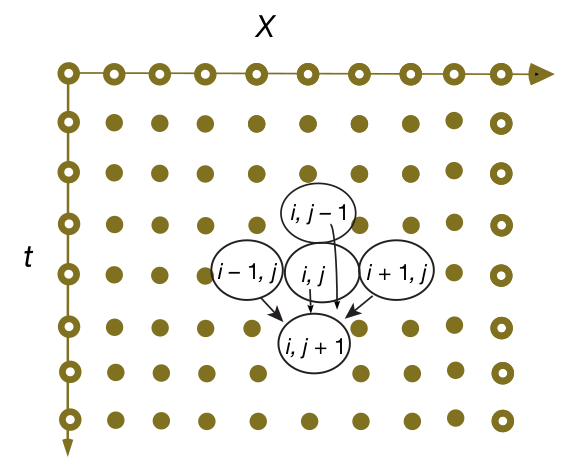
\includegraphics[width=20em]{compscieng_app17wave_03.png}

Yaklaşıksallıkta bir diğer kullanılacak teknik merkezi farklılıklar, burada $x$
için sola/sağa, $t$ için yukarı/aşağı olacak şekilde iki Taylor açılımı
yapıyoruz,


$$
y(x +\Delta x, t)  = y(x,t) +
\frac{\partial U}{\partial x}\Delta x + \frac{1}{2}
\frac{\partial^2 U}{\partial x^2}(\Delta x)^2 + \cdots
$$

$$
y(x -\Delta x, t)  = y(x,t) -
\frac{\partial U}{\partial x} \Delta x + \frac{1} {2}
\frac{\partial^2 U}{\partial x^2} (\Delta x)^2 - \cdots
$$

$$
y(x, y +\Delta t)  = y(x,t) +
\frac{\partial U}{\partial t}\Delta y + \frac{1}{2}
\frac{\partial^2 U}{\partial t^2}(\Delta t)^2 + \cdots
$$

$$
y(x, y -\Delta t) = y(x,t) -
\frac{\partial U}{\partial t} \Delta t + \frac{1} {2}
\frac{\partial^2 U}{\partial t^2} (\Delta t)^2 - \cdots
$$

Noktalı yerlerdeki terimleri yok sayıyoruz (2. derece yaklaşıklama yapmış olduk
yani, bu önemli, yaklaşık temsilin kuvvetini gösteriyor bir anlamda), sonra her
değişkenin iki açılımını birbiri ile topluyoruz. Toplama sonrası tek sayı
terimlerinin iptal olduğunu görürüz, ve kalanlar,

$$
\frac{\partial^2 y(x,t)}{\partial x^2} \simeq
\frac{y(x+\Delta x,t)+y(x-\Delta x,t)-2 y(x,t)}{(\Delta x)^2}
$$

$$
\frac{\partial^2 y(x,t)}{\partial t^2} \simeq
\frac{y(x,t+\Delta t) +y(x, y-\Delta t)-2 y(x,t)}{(\Delta t)^2}
$$

olacaktır. İndisler üzerinden belirtirsek,

$$
\frac{\partial^2 y }{\partial t^2} \simeq
\frac{y_{i,j+1}+y_{i,j-1}-2 y_{i,j}}{(\Delta t)^2}, \quad
\frac{\partial^2 y}{\partial x^2} \simeq
\frac{y_{i+1,j}+y_{i-1,j}-2 y_{i,j}} {(\Delta x)^2}.
$$

Üstteki formülleri dalga denklemindeki yerlerine koyarsak,

$$
\frac{y_{i,j+1}+y_{i,j-1}-2 y_{i,j}} {c^2 (\Delta t)^2}  =
\frac{y_{i+1,j}+y_{i-1,j}-2 y_{i,j}} {(\Delta x)^2}
$$

Tabii dikkat edersek geçmiş $j-1$ ve gelecek $j+1$ birbirine karışmış durumda,
bize lazım olan geleceğin hesabının eşitliğin sol tarafında olması geri kalan
her şey sağda olacak şekilde tekrar düzenlersek,

$$
y_{i,j+1}  = 2 y_{i,j}-y_{i,j-1}+ \frac{c^2 } {c'^{2}}
\left [ y_{i+1,j}+y_{i-1,j}-2 y_{i,j}\right], \quad c' { = }
\frac {\Delta x}{\Delta t}
\mlabel{1}
$$

Hesap için üstteki resmi hatırlayalım, $i,j+1$ hücresine dört diğer hücreden ok
çizilmiş, aslında bu oklar üstteki formülün hesabını anlatıyor, o anki $t$
zamanından üç hesap ve geçmişten $i,j-1$ hesabına bakarak gelecekteki değeri
hesaplıyoruz. Bu hesaplama çok verimli olacak çünkü herhangi bir anda hafızada
tutulması gereken $y(i,j)$ haricinde sadece üç tane değer var. 

Son bir problem başlangıç değerleriyle alakalı, resimdeki bilinmesi gereken o üç
hücrenin başlangıç $j=1$ anında olduğunu düşünürsek, ve $j=2$'yi hesaplamamız
gerekiyor, eksi zamana doğru bir gidişat lazım, yani $j=-1$ zamanı. Başlangıç
bilgisi $j=1$ var, ama $j=-1$ yok. Buradaki bilgiyi nasıl alacağız?

Denklemsel olarak bir ek koşul daha ekleyerek, ilk başta hem teli çekip üçgen
haline getirmiştik, bir de başlangıç anında telin hızı sıfırdır diyeceğiz. Bu
mantıksız değil, tel çekildi, tutuluyor.. hareket yok. Denklem olarak
$\partial y / \partial t(x,0)$ sıfır diyeceğiz. Sonra bu denklemin merkezi
farklılık açılımını yapacağız ve oradan gelen eşitlikleri ana (1)'e sokarak
sadece $j=2$ için özel bir formül elde etmeyi umuyoruz.

$$
\frac{\partial y}{\partial t}(x,0) \simeq
\frac{y(x, \Delta t)- y(x, -\Delta t)}{2\Delta t}=0, \
\Rightarrow \ y_{i, 0} = y_{i,2}
$$

(1)'e sokunca

$$
y_{i,2} = y_{i,1}+ \frac{c^2} {c'^2}
\left [ y_{i+1,1}+y_{i-1,1}-2 y_{i,1}\right]
$$

Dikkat bu denklem sadece $j=2$ için. Bundan sonraki her $j$ için ana (1) formülü
işleyecektir.

Stabilite, von Neumann

Çözümün stabil olması için $c \le \frac{\Delta x}{\Delta t}$ şartının doğru
olması gerekir, ve çoğunlukla $\Delta x$ bizim kontrolümüzde olmaz, problemin
dayattığı bir büyüklük olur, $c$ fiziki modelin bir parçasıdır, o zaman $\Delta t$'nin
diğer verili parametrelere göre şarta uygun seçilmesi gerekir. Şarta von
Neumann ya da Courant stabilite şartı ismi veriliyor.

Türetmek için alttaki gibi bir yaklaşım [3] kullanılabilir. Fakat ilerlemeden
önce Euler denkleminden türetilen bazı ek formülleri görelim, bu formüller
birazdan işimize yarayacak. Euler formülü hatırlarsak,

$$
e^{ix} = \cos (x) + i\sin(x)
$$

Üstteki formülü $-x$ için yazarsak,

$$
e^{-ix} = \cos (-x) + i\sin(-x)
$$

olur. Kosinüs'ün simetrik davranışı, yani $\cos(-x)=\cos(x)$ ve
$-\sin(x)=\sin(-x)$ olması sebebiyle, üstteki 

$$
= \cos(x) - i\sin(x)
$$

olarak yazılabilir. Şimdi eğer $e^{ix}$ ve $e^{-ix}$'i toplarsak, önceden
gördüğümüz açılımlar üzerinden,

$
e^{ix} + e^{-ix} = 2\cos(x)
$

olur, çünkü eksi işaretli $\sin$ artı olanla beraber iptal olur. Tekrar
düzenlersek,

$$
\cos(x) = \frac{1}{2} (e^{ix} + e^{-ix})
$$

Benzer bir eşitliği $e^{ix} - e^{-ix}$ üzerinden elde edebiliriz,

$$
e^{ix} - e^{-ix} = 2i\sin(x)
$$

Tekrar düzenleyince aynen biraz önce bir $\cos$ tanımı elde ettiğimiz gibi
bir de $\sin$ tanımı elde ederiz,

$$
\sin(x) = \frac{1}{2i} (e^{ix} - e^{-ix})
$$

Dalga kısmi denklemi ne idi?

$$
\partial_t^2 y(x,t) = c(x)^2 \partial_x^2 y(x,t)
$$

[2] notasyonu $c$ yerine $c(x)$ kullanmış. Şimdi stabilite şartını türetmek için
çözümün basit bir düzlem dalgası (plane wave) olduğunu farz edeceğiz [1], yani
çözüm

$$
y(x,t) = e^{i(kx-\omega t)}
$$

formunda olacak. Bu formu ayrıksallaştırıp kısmı türevsel forma sokunca çıkan
eşitlikler üzerinden bir stabilite şartı elde etmek amacımız. [3] notasyonu
yerine [2]'imsi notasyon kullanacağız, yani $x,t$ indisleri $i,j$ yerine $j,n$,
herhalde hayali sayı $i$ ile karışıklık olmasın diye böyle seçilmiş. O zaman $x
\to j \Delta x$, $t \to n \Delta t$ olur.

Alttaki analitik soldaki formül ayrıksal şu hale gelir,

$$
y(x,t) = e^{i(kx - \omega t)} \to
y_{j,n} = e^{i(kj\Delta x - \omega n \Delta t)}
$$


[devam edecek]

Kaynaklar

[1] Bayramlı, {\em Fizik, Isı ve Dalga Denklemleri}

[2] Igel, {\em Computers, Waves, Simulations, Coursera Lecture, Week 3, von Neumann Analysis},
    \url{https://www.coursera.org/learn/computers-waves-simulations}

[3] Landau, {\em Landau Computational Physics Course, Video Lectures},
    \url{https://www.youtube.com/playlist?list=PLnWQ_pnPVzmJnp794rQXIcwJIjwy7Nb2U}


\end{document}
